\documentclass[letterpaper,headings=standardclasses]{scrartcl}

\usepackage[margin=1in,includefoot]{geometry}
\usepackage{amssymb}
\usepackage{amsmath}
\usepackage{listings}
\usepackage{tikz}
\usepackage{float}
\usepackage{algorithm}
\usepackage{algpseudocode}

\DeclareMathOperator*{\argmax}{argmax}
\DeclareMathOperator*{\argmin}{argmin}

\usetikzlibrary{shapes,arrows}

\tikzset{
  block/.style    = {draw, thick, rectangle, minimum height = 3em, minimum width = 3em},
  sum/.style      = {draw, circle},
  input/.style    = {coordinate, circle},
  output/.style   = {coordinate, circle}
}

\lstset{basicstyle=\ttfamily,language=python,columns=flexible,breaklines=true,showstringspaces=false}

\title{Homework 5}
\subtitle{CS 559 - Neural Networks - Fall 2019}
\author{Matteo Corain 650088272}

\begin{document}

\maketitle

\section{Question 1}

\subsection{Data parsing and preprocessing}

Data have been parsed from the images and label files using a variation of the functions defined in the second homework for this purpose. Specifically:

In order to parse the images and labels files, two separate functions have been coded:

\begin{itemize}

    \item Function \texttt{idx\_images\_parse()} is used to parse the images files encoded in the IDX format; it performs the following actions:

        \begin{itemize}

        \item It opens the given file in \emph{read binary} mode;

        \item It reads the magic number using the \texttt{fromfile()} function provided by the Numpy library, which allows to read a certain number of elements (in this case, a single one) from a file given their data type (in this case, big endian \texttt{>}, unsigned integer \texttt{u} on four bytes \texttt{4}) and checks its correctness (it must be equal to 2051);

        \item In the same way, it reads the number of items and the dimensions of the input images into variables \texttt{n\_samples}, \texttt{n\_rows} and \texttt{n\_cols};

        \item Using the list comprehension syntax and the \texttt{fromfile()} function provided by the Numpy library, it reads \texttt{n\_samples} arrays of \texttt{n\_rows * n\_cols} elements stored as big endian, unsigned 8-bits integers (\texttt{>u1}), reshapes them to the correct format and stores them into the \texttt{samples} variable;

        \item It returns variables \texttt{n\_samples}, \texttt{n\_rows}, \texttt{n\_cols} and \texttt{samples}.

        \end{itemize}

    \item Function \texttt{idx\_labels\_parse()} is used to parse the labels files encoded in the IDX format; it performs similar actions with respect to the previous one, the only differences being that in this case samples dimensions are not present and that data items are represented by single 8-bits elements.

\end{itemize}

With respect to the functions used for the second homework, some preprocessing is done on the data before feeding them to the network as training samples. In particular, the following preprocessing has been applied:

\begin{itemize}

    \item Input pixel values have been normalized to 1, by dividing each component by 255 (they are stored as 8-bits unsigned integers), after subtracting them their mean value (so that they have zero mean);
    
    \item Labels have been mapped on their binary vector representation, using the \texttt{label\_to\_array()} function from homework 2.

\end{itemize}

Scaling the inputs allows for avoiding the need of training large weights for the network, while label mapping is useful since it is not necessary to reconstruct the binary representation each time it is needed (it is computationally easier to extract the argmax, when necessary).

\subsection{Hyperparameters selection}

For the purpose of the exercise, the networks to be tested have been chosen according to the following parameters:

\begin{itemize}
    
    \item \emph{Network topology}: as for the network topology, all the considered networks are either 2-layers or 3-layers. The choice of not using more than 3 layers has been dictated both by the computational complexity that the training of multiple layers yields and by the fact that, in any case, a 2-layers network is already capable of approximating any function with arbitrary precision. The addition of a second hidden layer is motivated by the willingness to compare the training performance of multiple-layers networks with respect to the 2-layers ones.
    
    \item \emph{Digit representation}: classified digits have been represented as in homework 2; for this reason, all the tested networks present 10 neurons in the output layer, and the class prediction is obtained by extracting the argmax of the network output. This representation is in fact handy because it allows also to assign a form of "confidence score" to the different predictions that the network returns (i.e. the network classifies the input pattern as an $i$ digit with a confidence given by $y_i$).
    
    \item \emph{Activation functions}: as for activation functions, it has been chosen to utilize hyperbolic tangents for the hidden layers and sigmoid for the output layer. Hyperbolic tangents have been chosen for their well-known properties that make them suitable for the usage in neural networks (e.g. they are odd functions), while sigmoids have been used in order to saturate the network output in a positive range between 0 and 1, allowing to interpretate results as a sort of "probabilistic" confidence score (not really true since they do not sum to 1).
    
    \item \emph{Learning rates}: for the sake of simplicity, all neurons in the networks make use of the same learning rate $\eta$, initially set to a reasonable $\eta = 0.01$. A dynamic update mechanism of the learning rate has also been implemented, decrementing the value of $\eta$ by a factor of 0.9 each time it comes across an increase of the error function from an epoch to the following.
    
    \item \emph{Energy function}: the mean squared error measure has been chosen as the energy function for all the tested networks:
    
    $$ E = \frac{1}{|\mathcal{S}|} \sum_{i = 1}^{|\mathcal{S}|} || d_i - y_{i,L} ||^2 $$
    
    \item Other implementation heuristics:
    
    \begin{itemize}
        \item \emph{Stochastic update}: online learning has been used for all training tasks;
        \item \emph{Inputs normalization}: inputs have been scaled in the range $[0,1]$ to avoid saturation;
        \item \emph{Weights initialization}: weight matrices have been initialized using random values drawn from a normal distribution with $\mu = 0$ and $\sigma = m^{-1}$, where $m$ represents the number of inputs of each specific layer.
    \end{itemize}

\end{itemize}

\subsection{Network construction and training}

In order to properly represent the different networks, a \texttt{Network} class has been defined. Its constructor takes as arguments three lists, the first one containing the initial weights matrices (biases included) of each layer of the network, the second containing the function pointers corresponding to the activation functions of each layer of the network and the third the function pointers of the derivatives thereof. The class presents the following methods:

\begin{itemize}

    \item \texttt{feedforward()}: it feeds the network with the input $x = y_0$, computing for each layer the corresponding value of the local field $v$ and of the output $y$:
    
    $$ v_i = W_i \left[ \begin{matrix} 1 \\ y_{i - 1} \end{matrix} \right] $$
    $$ y_i = \phi_i(v_i) $$
    
    \item \texttt{backpropagate()}: it estimates the value of the gradient of the energy function $\nabla E$ through the backpropagation algorithm, for an input pattern $x$ with desired output $d$; this is performed in three steps:
    
    \begin{itemize}

        \item In the first step, the $v$ and $y$ vectors of the induced fields and outputs of each neuron are computed through the \texttt{feedforward()} method;

        \item In the second step, the delta signals are calculated, in reverse order of $i$:
        
        $$ \delta_L = (d - y_L) \cdot \phi'_L(v_L) $$
        $$ \delta_i = \underline{W_{i + 1}^T} \delta_{i + 1} \cdot \phi'_i(v_i), i = L - 1, \dots, 1 $$

        Where the underline denotes the weight matrix in which the first row (the one related to the bias term) has been removed.

        \item In the third step, delta signals are used to compute the effective components of the desired gradient:
        
        $$ \frac{\partial E}{\partial W_i} = -\delta_i \left[ \begin{matrix} 1 \\ y_{i - 1} \end{matrix} \right] $$

    \end{itemize}
    
    \item \texttt{error()}: it calculates the value of the error function for the entire training set (mean squared error), averaging the squared value of the norm of the difference between the desired outputs and the effective outputs (computed through the \texttt{feedforward()} method):
    
    $$ E = \frac{1}{|\mathcal{S}|} \sum_{i = 1}^{|\mathcal{S}|} || d_i - y_{i,L} ||^2 $$
    
    \item \texttt{test()}: it calculates the accuracy of the network on the test set, by summing a value of 1 each time the classification is correct (that is, $ \argmax{y_{i,L}} = \argmax{d_i} $) and dividing by the number of test samples:
    
    $$ a = \frac{1}{|\mathcal{T}|} \sum_{i = 1}^{|\mathcal{T}|} \alpha_i, \; \alpha_i = \begin{cases} 1 & \text{if } \argmax{y_{i,L}} = \argmax{d_i} \\ 0 & \text{otherwise} \end{cases} $$
    
    \item \texttt{train()}: it performs a gradient descent, backpropagation-based training of the network; it takes as parameters:
    
    \begin{itemize}

        \item The training samples and labels;
        \item The test samples and labels (to record the test set accuracy for increasing epochs);
        \item The initial learning rate $\eta$;
        \item The target value of the error function $\epsilon$;
        \item The batch size for the learning procedure;
        \item A string suffix to be used for storing computed quantities in appropriate files for later usage (e.g. plotting) without having to fully recompute them.
    
    \end{itemize}

    The procedure performs the following actions:

    \begin{itemize}
        
        \item It initializes the \texttt{errors} and \texttt{tests} lists with the initial values of the error function and of the test set accuracy;
        
        \item It enters the training loop, whose stopping conditions are expressed on the number of epochs (it has to be lower than the configured limit) and on the value of the error function (it has to be greater than the configured limit);
        
        \item It loops on the training samples, computing for each of them the value of $\nabla E$ through the \texttt{backpropagate()} method, then updates the weight matrices of the different layers using the standard gradient descent rule;
        
        \item It registers the value of the error function and the accuracy on the test set for the current weights;
        
        \item If the value of the error function increases among two consecutive epochs, it reduces the learning rate of a factor of 0.9.
        
        \item When the training loop is computed, the final weights and the lists of errors and accuracy values are saved to file and returned.

    \end{itemize}

\end{itemize}

\begin{algorithm}[H]
    \caption{Feed-forward procedure}
    \label{ffalg}
    \begin{algorithmic}
    
    \Function{Feed-Forward}{$network, x_i$}
        \State \Comment{Initialization}
        \State $v \gets $ \Call{Empty-List}{}
        \State $y \gets $ \Call{Empty-List}{}
        \State $y[0] \gets x_i$
        \State \Comment{Computation of $v$ and $y$ values}
        \For{$i = 1, \dots, L$}
            \State $v[i] \gets network.W[i] \left[ \begin{matrix} 1 & y[i] \end{matrix} \right]^T$
            \State $y[i + 1] \gets network.\phi[i](v[i])$
        \EndFor
        \State \Return $v, y$
    \EndFunction

    \end{algorithmic}
\end{algorithm}

\begin{algorithm}[H]
    \caption{Backpropagation procedure}
    \label{bpalg}
    \begin{algorithmic}
    
    \Function{Backpropagate}{$network, x_i, d_i$}
        \State \Comment{Initialization}
        \State $v, y \gets network.\Call{Feed-Forward}{x_i}$
        \State $\delta \gets $ \Call{Empty-List}{}
        \State $\nabla E \gets $ \Call{Empty-List}{}
        \State \Comment{Computation of $\delta_i$ values}
        \State $\delta[L] \gets (d_i - y[L]) * network.\phi'[L](v[L])$
        \For{$i = L - 1, \dots, 1$}
            \State $\delta[i] \gets \left( network.\underline{W[i + 1]} \right)^T \delta[i + 1] * network.\phi'[i](v[i])$
        \EndFor
        \State \Comment{Computation of $\nabla E$ components}
        \For{$i = 1, \dots, L$}
            \State $\nabla E[i] = -\delta[i] \left[ \begin{matrix} 1 & y_{i - 1} \end{matrix} \right]^T$
        \EndFor
        \State \Return $v, y$
    \EndFunction
    
    \end{algorithmic}
\end{algorithm}

\begin{algorithm}[H]
    \caption{Error procedure}
    \label{eralg}
    \begin{algorithmic}
    
    \Function{Error}{$network, x, d$}
        \State $e \gets 0$
        \For{$i = 1, \dots, n$}
            \State $v, y \gets network.\Call{Feed-Forward}{x[i]}$
            \State $e \gets e + (d[i] - y[L])^2$
        \EndFor
        \State \Return $e / n$
    \EndFunction
    
    \end{algorithmic}
\end{algorithm}

\begin{algorithm}[H]
    \caption{Test procedure}
    \label{ttalg}
    \begin{algorithmic}
    
    \Function{Test}{$network, x, d$}
        \State $c \gets 0$
        \For{$i = 1, \dots, n$}
            \State $v, y \gets network.\Call{Feed-Forward}{x[i]}$
            \If{$\argmax{d[i]} = \argmax{y[L]}$}
                \State $c \gets c + 1$
            \EndIf
        \EndFor
        \State \Return $c / n$
    \EndFunction
    
    \end{algorithmic}
\end{algorithm}

\begin{algorithm}[H]
    \caption{Training procedure}
    \label{tralg}
    \begin{algorithmic}
    
    \Function{Train}{$network, x_{train}, d_{train}, x_{test}, d_{test}, \eta, \epsilon, \lambda$}
        \State \Comment{Initialization}
        \State $epochs \gets 0$
        \State $errors \gets $ \Call{Empty-List}{}
        \State $trainacc \gets $ \Call{Empty-List}{}
        \State $testacc \gets $ \Call{Empty-List}{}
        \State $errors[0] \gets network.\Call{Error}{x_{train}, d_{train}}$
        \State $trainacc[0] \gets network.\Call{Error}{x_{train}, d_{train}}$
        \State $testacc[0] \gets network.\Call{Error}{x_{test}, d_{test}}$
        \State \Comment{Main weights update loop}
        \While{$epochs < \lambda \wedge errors[epochs] > \epsilon$}
            \State $epochs \gets epochs + 1$
            \State \Comment{Compute update terms and update weights}
            \For{$i = 1, \dots, n$}
                \State $\nabla E \gets network.\Call{Backpropagate}{x_{train}[i], d_{train}[i]}$
                \For{$j = 1, \dots, L$}
                    \State $network.W[j] \gets network.W[j] - \eta \nabla E[j]$
                \EndFor
            \EndFor
            \State \Comment{Error and accuracy registration}
            \State $errors[epochs] \gets network.\Call{Error}{x_{train}, d_{train}}$
            \State $trainacc[epochs] \gets network.\Call{Error}{x_{train}, d_{train}}$
            \State $testacc[epochs] \gets network.\Call{Error}{x_{test}, d_{test}}$
            \State \Comment{Update of $\eta$}
            \If{$errors[epochs] > errors[epochs - 1]$}
                \State $\eta \gets 0.9 \eta$
            \EndIf
        \EndWhile
        \State \Return $epochs, errors, trainacc, testacc$
    \EndFunction
    
    \end{algorithmic}
\end{algorithm}

\subsection{Tested networks and results}

For the sake of the exercise, six networks have been tested, whose main parameters are presented in table \ref{net_params}.

\begin{table}[h]
    \centering
    \begin{tabular}{|c|c|c|c|c|c|c|c|c|c|c|}
    \hline
    Network \# & Layers & $n_1$ & $n_2$ & $n_3$ & $\phi_1$ & $\phi_2$ & $\phi_3$ & $\eta$ & $\epsilon$ & Epoch limit \\ \hline
    1 & 2 & 10 & 10 & - & tanh & sigmoid & - & 0.01 & 0.01 & 100 \\ \hline
    2 & 2 & 100 & 10 & - & tanh & sigmoid & - & 0.01 & 0.01 & 100 \\ \hline
    3 & 2 & 200 & 10 & - & tanh & sigmoid & - & 0.01 & 0.01 & 100 \\ \hline
    4 & 3 & 10 & 10 & 10 & tanh & tanh & sigmoid & 0.01 & 0.01 & 100 \\ \hline
    5 & 3 & 100 & 10 & 10 & tanh & tanh & sigmoid & 0.01 & 0.01 & 100 \\ \hline
    6 & 3 & 100 & 100 & 10 & tanh & tanh & sigmoid & 0.01 & 0.01 & 100 \\ \hline
    \end{tabular}
    \caption{Parameters of the tested networks}
    \label{net_params}
\end{table}

For the selection of the number of neurons for each layer of each network, it has been chosen to start from the network used for this classification task in homework 2. In that case, we made use of a single-layer network with 10 neurons, capable of achieving an accuracy of about 85\% when trained using the whole training set.

For this reason, a first try was performed, using a 2-layers network having the same number of neurons (10) for both the hidden and the output layer. Despite such network has not been able to converge to the configured maximum error value within the configured number of epochs, the training performances of such network already show a sensible improvement over the network used in homework 2 (93.79\% accuracy for the training set, 91.79\% accuracy for the test set).

Given that the precision of the approximation of a 2-layer network may be improved by introducing additional neurons, it has then been chosen to test two additional 2-layers networks, having respectively 100 and 200 neurons in their hidden layer. These networks performed much better, reaching convergence in 63 and 43 epochs respectively with around 99.5\% training set accuracy and almost 98\% test set accuracy. The downside for that has been the significant increase in training time, especially for the network with 200 elements in the hidden layer.

For the 3-layers network, a similar process has been followed. Initially, it has been chosen to test the performance of a network having 10 neurons in both hidden layers, the training of which again reached the configured epoch limit; as expected, the performance of such network are better than the ones of the initial 2-layers network due to the increased abstraction capabilities introduced by the additional hidden layer, but still not in line with the 95\% test set accuracy target (95.44\% for the training set, 92.87\% for the test set).

Again, two additional 3-layers networks have been tested, increasing the number of neurons respectively in the first and in both hidden layers. Those networks were the ones that yielded the best performances in terms of training epochs and time overall, reaching accuracy levels comparable to the ones of 2-layers networks, with a reduction of about half for the number of training epochs and of 3 to 4 times for the training time.

A summary of the results of the training process are shown in table \ref{net_results}. The overall best network, in terms of ratio between accuracy and training time is the 100-10-10 one, although the 100-100-10 converges in a more limited number of epochs.

\begin{table}[h]
    \centering
    \begin{tabular}{|c|c|c|c|c|}
    \hline
    Network \# & Epochs & Training time (s) & Training set accuracy & Test set accuracy \\ \hline
    1 & 100+ & 913 & 93.79\% & 91.79\% \\ \hline
    2 & 63 & 3486 & 99.46\% & 97.62\% \\ \hline
    3 & 43 & 7704 & 99.54\% & 97.90\% \\ \hline
    4 & 100+ & 1130 & 95.44\% & 92.87\% \\ \hline
    5 & 29 & 1366 & 99.48\% & 97.54\% \\ \hline
    6 & 24 & 2303 & 99.50\% & 98.00\% \\ \hline
    \end{tabular}
    \caption{Training results for the tested networks}
    \label{net_results}
\end{table}

Figures \ref{errors_plot}, \ref{trains_plot} and \ref{tests_plot} show respectively the value of the error function, the training set and the test set accuracy for increasing number of epochs for the considered networks (epoch 0 is excluded because significantly out-of-scale). It is possible to notice how the performances of network 3 are consistently better than the ones of network 2, which in turn has better performances than network 1, throughout the entire learning process.

\begin{figure}[H]
    \centering
    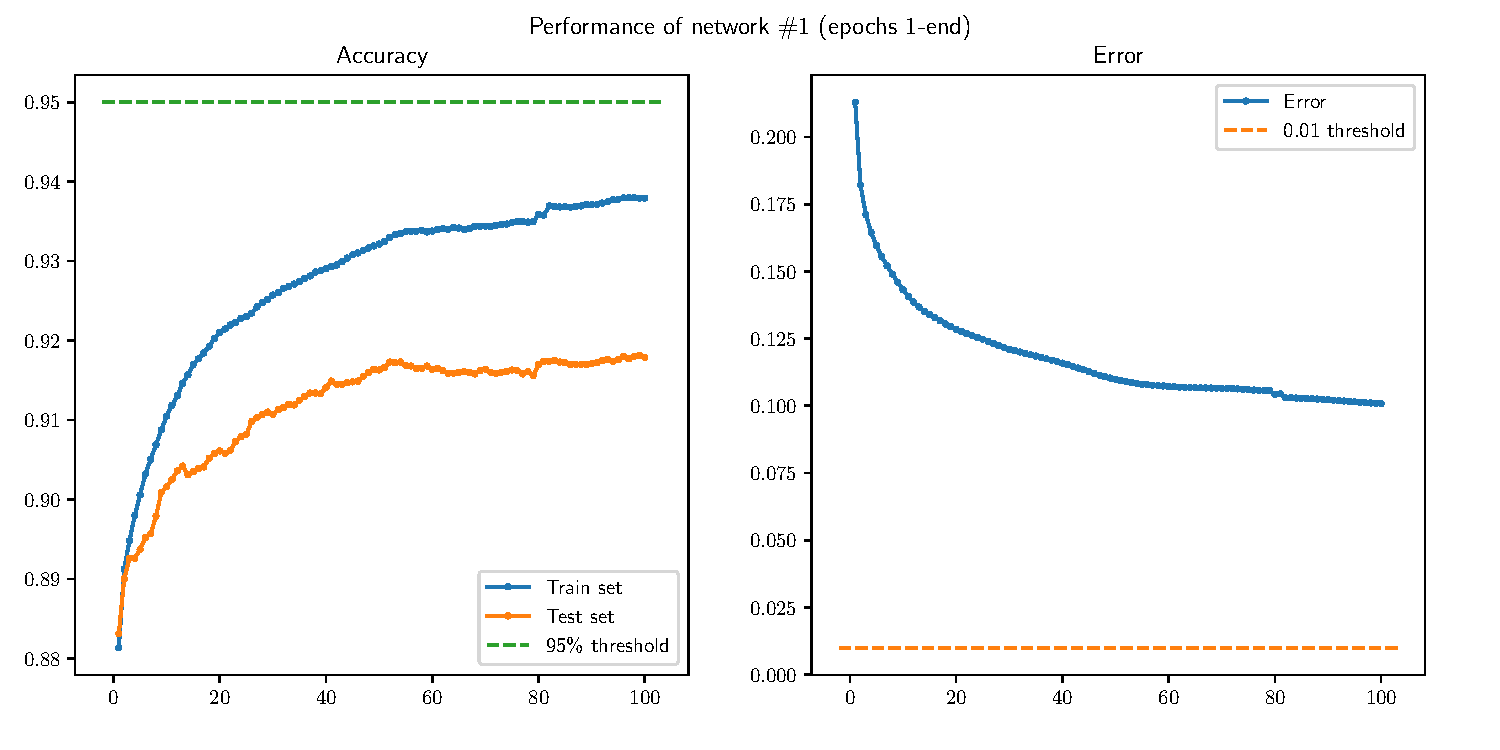
\includegraphics[width=\linewidth]{net1.pdf}
    \caption{Performances of network \#1}
    \label{net1}
\end{figure}

\begin{figure}[H]
    \centering
    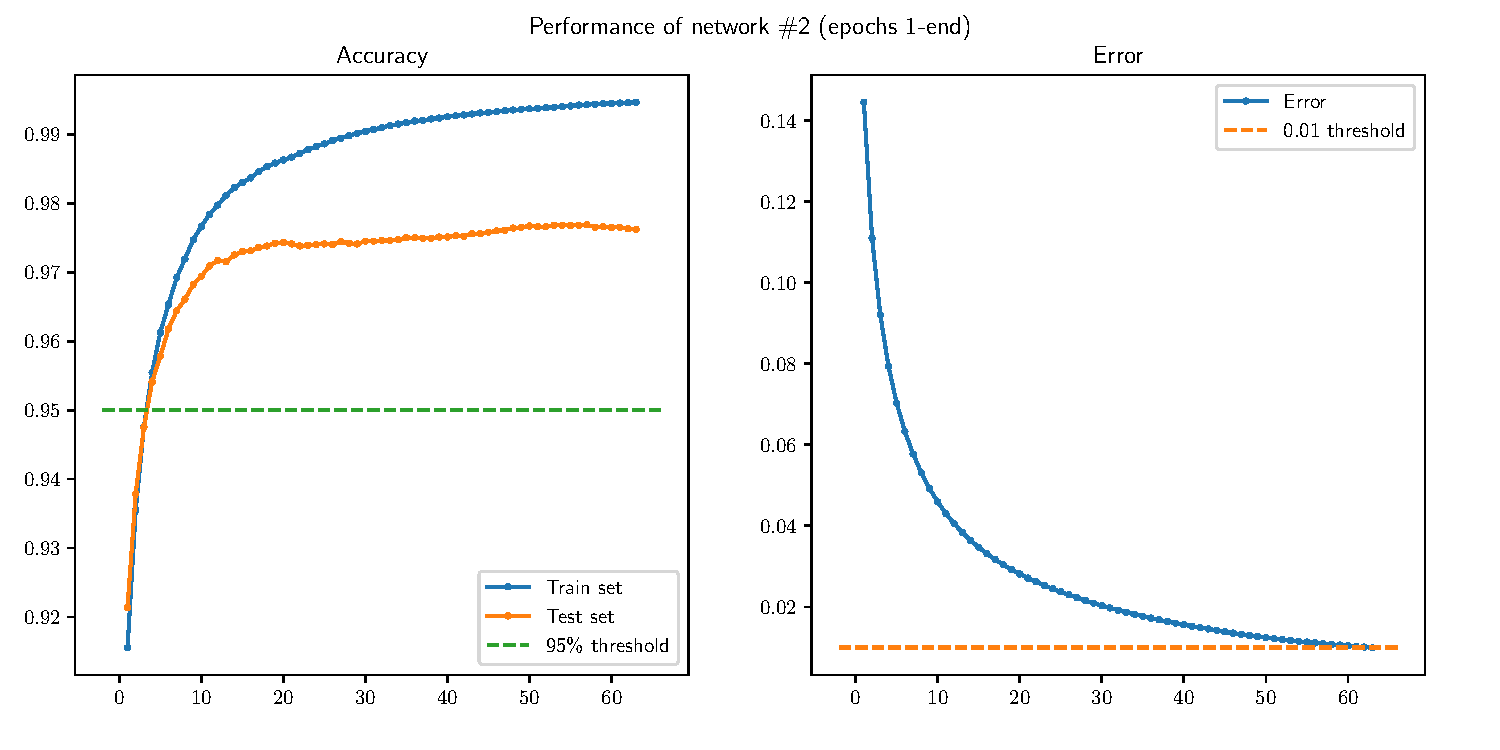
\includegraphics[width=\linewidth]{net2.pdf}
    \caption{Performances of network \#2}
    \label{net2}
\end{figure}

\begin{figure}[H]
    \centering
    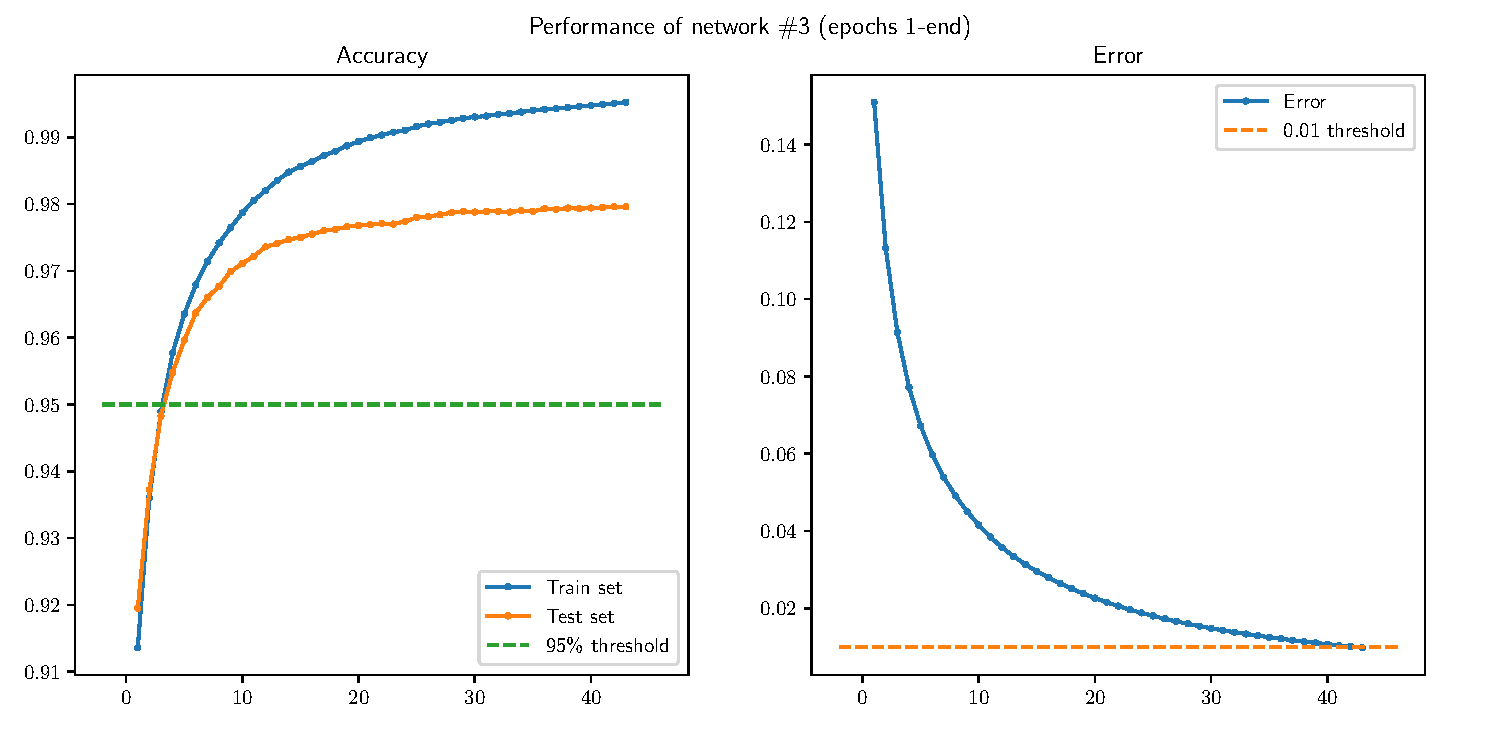
\includegraphics[width=\linewidth]{net3.pdf}
    \caption{Performances of network \#3}
    \label{net3}
\end{figure}

\begin{figure}[H]
    \centering
    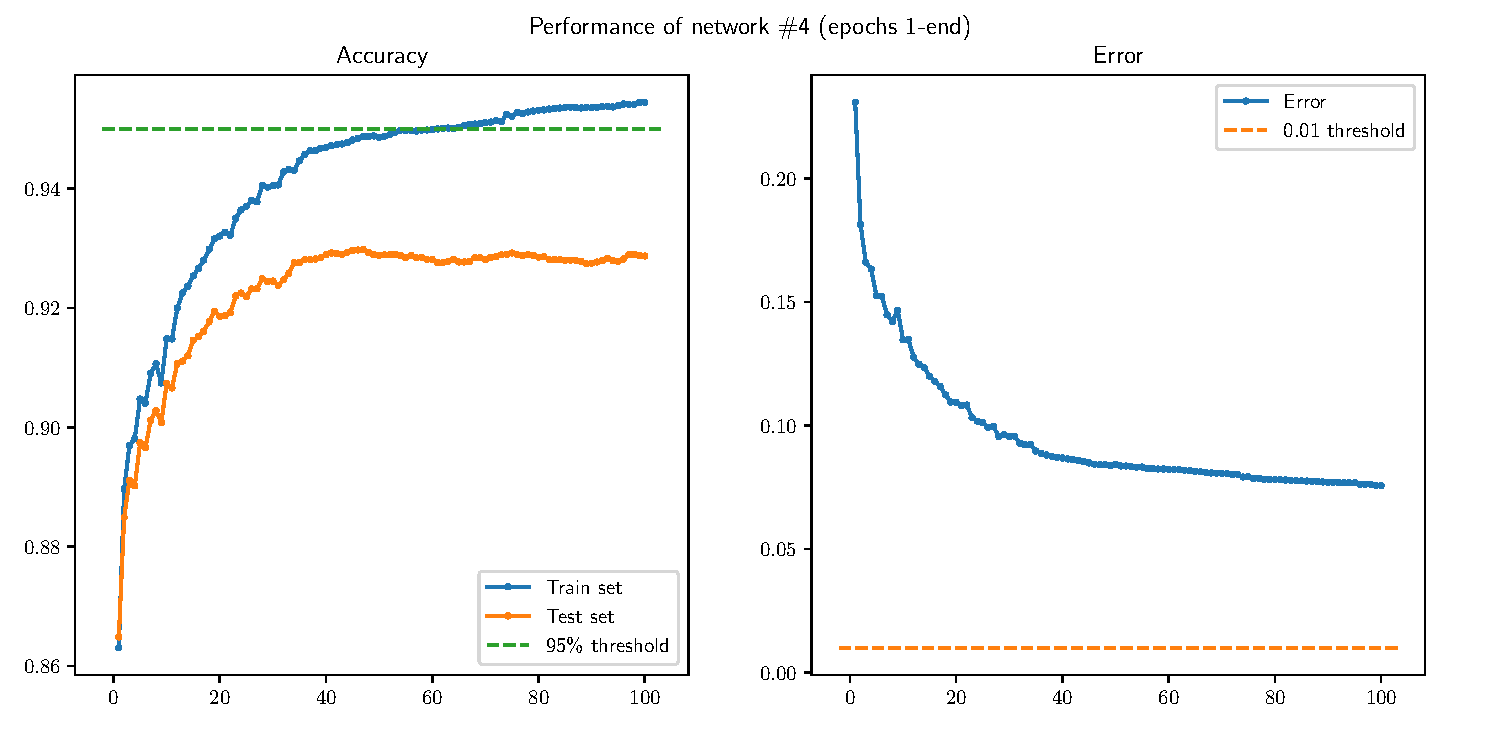
\includegraphics[width=\linewidth]{net4.pdf}
    \caption{Performances of network \#4}
    \label{net4}
\end{figure}

\begin{figure}[H]
    \centering
    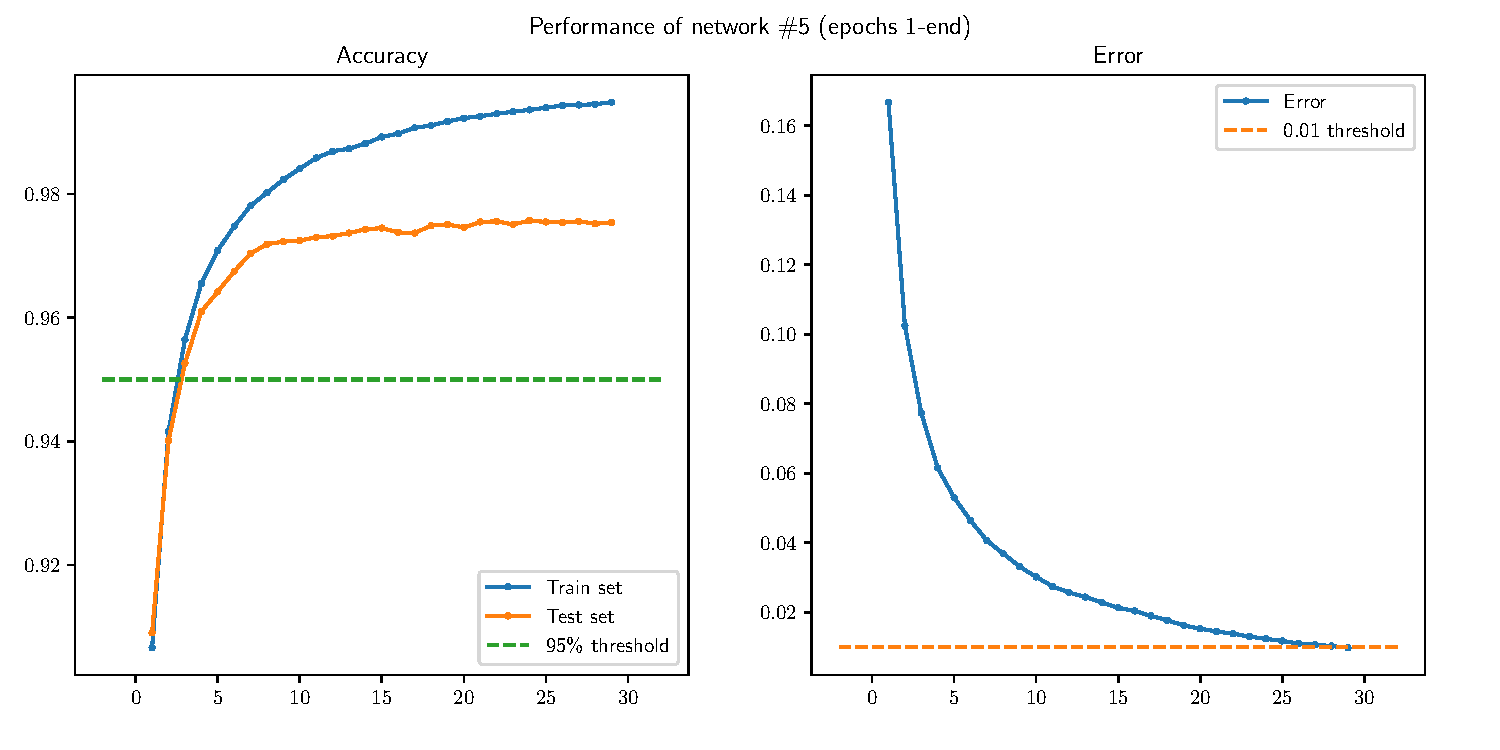
\includegraphics[width=\linewidth]{net5.pdf}
    \caption{Performances of network \#5}
    \label{net5}
\end{figure}

\begin{figure}[H]
    \centering
    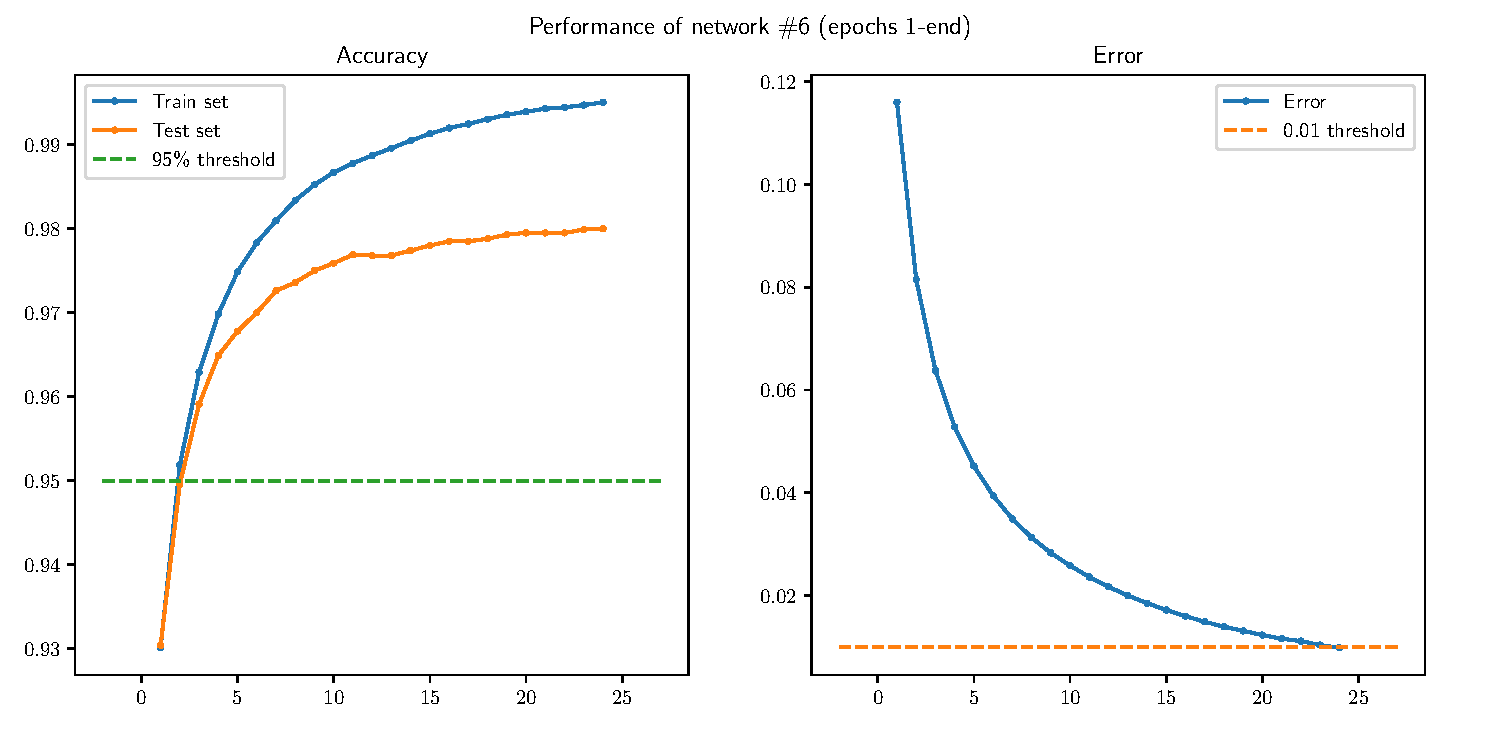
\includegraphics[width=\linewidth]{net6.pdf}
    \caption{Performances of network \#6}
    \label{net6}
\end{figure}

\subsection{Complete Python code}

\subsubsection{Data parsing functions}

\lstinputlisting[basicstyle=\ttfamily\scriptsize]{idxfuncs.py}

\subsubsection{Network class definition}

\lstinputlisting[basicstyle=\ttfamily\scriptsize]{network.py}

\subsubsection{Training of the networks}

\lstinputlisting[basicstyle=\ttfamily\scriptsize]{hw5.py}

\end{document}